\newpage
\subsection{\vertex}
\secwriter{A. Zupanc}

\paragraph{General overview} This class represents the reconstructed vertices, e.g.
\begin{itemize}
 \item $B_{\rm tag}$ vertex is in $t$-dependent studies,
 \item production vertices determined as a crossing of particle's trajectory with the IP region (used in charm studies),
 \item vertex determined as a crossing of two or more charged particles's trajectories
\end{itemize}

Note, that in general the decay vertices of exclusively reconstructed decays are stored inside the \particle object and there is
no need to create and store the \vertex object in the \dStore in such case (therefore the decay vertex is not mentioned above as 
an use-case of the \vertex class). 

If it is found usefull, the \vertex object can be related with \basf\ \relation to the \particle objects which were fitted
together to form this vertex (this feature is {\it for free} in \basf).

\subsubsection{Data members}

\paragraph{Persistent members}
\begin{itemize}
 \item {\color{blue}position} \hfill{$3\times$float}
 \item {\color{blue}$3\times3$ error matrix} \hfill{$6\times$float}
 \begin{itemize}
  \item order of elements in error matrix is: $x,y,z$
  \item internally the error matrix is saved as one dimensional array with 6 elements
 \end{itemize}
 \item {\color{blue} $\chi^2$ value of the fit} \hfill{float}
 \item {\color{blue}number of degrees of freedom of the fit} \hfill{unsigned}
\end{itemize}

\paragraph{Transient members} This class has no transient data members.

\subsubsection{Constructors}

\begin{itemize}
 \item {\bluett Vertex(TVector3, TMatrixFSym, float, unsigned)}
 \begin{itemize}
  \item all private members are initialized to the values passed as constructor arguments
 \end{itemize}
\end{itemize}

\subsubsection{Member functions}

\paragraph{Getters/Setters for private members}

The table given below provides list of available getters and setters for private members:
\begin{center}
 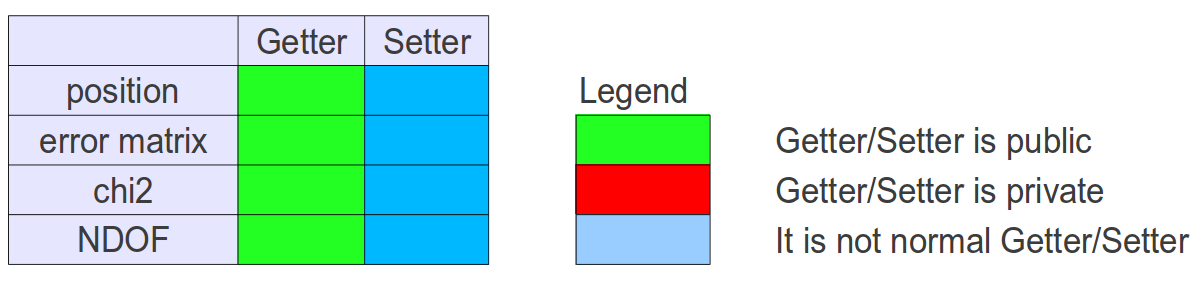
\includegraphics[width=0.9\textwidth]{DataModel/figs/vertexGetterSetter.png}
\end{center}
The getters return position and its error matrix as {\tt TVector3} and {\tt TMatrixFSym}, 
respectively. 

Single public function is provided which updates all private members at once:
\begin{itemize}
 \item {\bluett updateVertex(TVector3, TMatrixFSym, float, unsigned)}
\end{itemize}
